% This LaTeX was auto-generated from MATLAB code.
% To make changes, update the MATLAB code and export to LaTeX again.

\documentclass{article}

\usepackage[utf8]{inputenc}
\usepackage[T1]{fontenc}
\usepackage{lmodern}
\usepackage{graphicx}
\usepackage{color}
\usepackage{hyperref}
\usepackage{amsmath}
\usepackage{amsfonts}
\usepackage{epstopdf}
\usepackage[table]{xcolor}
\usepackage{matlab}

\sloppy
\epstopdfsetup{outdir=./}
\graphicspath{ {./selfconsistency_images/} }

\begin{document}

\label{H_F310D61F}
\matlabtitle{Self-Consistent Order Parameter}


\vspace{1em}
\matlabheading{BCS Hamiltonian with magnetic field}

\begin{par}
\begin{flushleft}
The BCS Hamiltonian with Peierls substitution can be generated with \texttt{bcsRectangularCell(in)}.
\end{flushleft}
\end{par}

\begin{par}
\begin{flushleft}
\texttt{in }is a structure consisting of elements:
\end{flushleft}
\end{par}

\begin{par}
\begin{flushleft}
\texttt{Nx, Ny - System lengths}
\end{flushleft}
\end{par}

\begin{par}
\begin{flushleft}
\texttt{chemPot - Chemical potential}
\end{flushleft}
\end{par}

\begin{par}
\begin{flushleft}
\texttt{hopInt - Hopping integral}
\end{flushleft}
\end{par}

\begin{par}
\begin{flushleft}
\texttt{b - Magnetic field strength scaled with }$2\pi$
\end{flushleft}
\end{par}

\begin{par}
\begin{flushleft}
\texttt{impurityArray - An array of potential impurities, major order along x}
\end{flushleft}
\end{par}

\begin{par}
\begin{flushleft}
\texttt{gapArray - An array of on-site SC order parameter, major order along x}
\end{flushleft}
\end{par}


\vspace{1em}
\matlabheading{SC Order Parameter}

\begin{par}
\begin{flushleft}
The superconducting order parameter can be calculated with \texttt{calcGap(V, T, P, eigenP)}.
\end{flushleft}
\end{par}

\begin{par}
\begin{flushleft}
\texttt{V - Attractive potential (positive value)}
\end{flushleft}
\end{par}

\begin{par}
\begin{flushleft}
\texttt{T - Temperature}
\end{flushleft}
\end{par}

\begin{par}
\begin{flushleft}
\texttt{P - Unitary transformation matrix of BCS Hamiltonian}
\end{flushleft}
\end{par}

\begin{par}
\begin{flushleft}
\texttt{eigenP - Diagonalized matrix of BCS Hamiltonian }
\end{flushleft}
\end{par}


\vspace{1em}
\matlabheading{Filling}

\begin{par}
\begin{flushleft}
The filling can be calculated with \texttt{calcN(T, P, eigenP)}.
\end{flushleft}
\end{par}

\begin{par}
\begin{flushleft}
\texttt{T - Temperature}
\end{flushleft}
\end{par}

\begin{par}
\begin{flushleft}
\texttt{P - Unitary transformation matrix of BCS Hamiltonian}
\end{flushleft}
\end{par}

\begin{par}
\begin{flushleft}
\texttt{eigenP - Diagonalized matrix of BCS Hamiltonian }
\end{flushleft}
\end{par}


\vspace{1em}
\matlabheading{Calculating the self consistent SC order parameter}


\vspace{1em}
\matlabheadingtwo{Parameter initialization}

\begin{par}
\begin{flushleft}
Initialize parameters in a structure, i.e. with \texttt{tDependencePar.m} where  \texttt{in} struct is created to a data.
\end{flushleft}
\end{par}

\matlabheadingtwo{Convergence algorithm}

\begin{par}
\begin{flushleft}
Use \texttt{varCalc(in, tFactor) }to use fixed point iteration to find self-consistent SCOP for a particular temperature \texttt{tFactor} up to a maximum iteration \texttt{in.maxIterations}.
\end{flushleft}
\end{par}

\matlabheadingtwo{Examples}

\matlabheadingthree{Temperature dependence}

\begin{par}
\begin{flushleft}
One can sweep \texttt{varCalc()} over different temperature. Use \texttt{tDependencePar.m} to initialize and \texttt{tDependence.m} to iterate over the defined interval of temperature.
\end{flushleft}
\end{par}

\begin{par}
\begin{flushleft}
Temperature dependence can be fitted with the theoretical gap equation through \texttt{gapEquation(T,MaxGap,Tc)} where \texttt{MaxGap} and \texttt{Tc} are the fitting parameters :
\end{flushleft}
\end{par}

\begin{matlabcode}
run('FitAndPlotGapT.m')
\end{matlabcode}
\begin{matlaboutput}
Local minimum possible.

lsqcurvefit stopped because the final change in the sum of squares relative to 
its initial value is less than the value of the function tolerance.

<stopping criteria details>
\end{matlaboutput}
\begin{center}
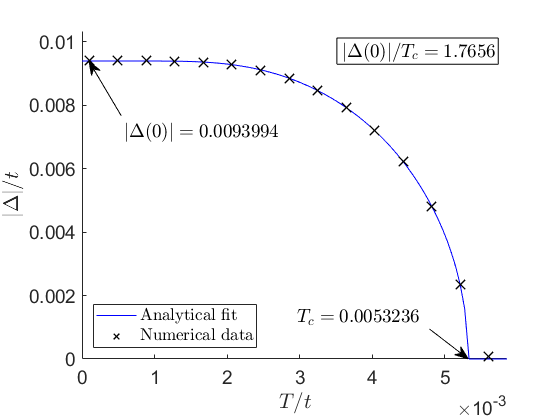
\includegraphics[width=\maxwidth{56.196688409433015em}]{figure_0.png}
\end{center}

\matlabheadingthree{Order parameter time series}

\begin{par}
\begin{flushleft}
For saving the history of the SCOP, we can use \texttt{vortexEvolution(filename\_in,filename\_out)}. This tracks the gap parameter for 20 evenly-divided intervals of iterations from the given maximum iterations. The parameters are initialized with \texttt{trackPar.m}.
\end{flushleft}
\end{par}

\begin{par}
\begin{flushleft}
Different plots can be generated, i.e.
\end{flushleft}
\end{par}

\begin{par}
\begin{flushleft}
Convergence of SCOP:
\end{flushleft}
\end{par}

\begin{matlabcode}
run('convergencePlot.m')
\end{matlabcode}
\begin{center}
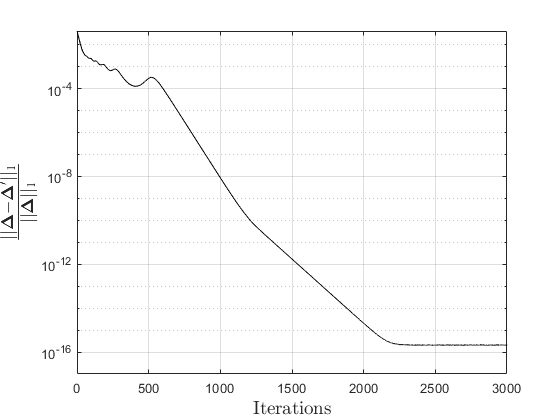
\includegraphics[width=\maxwidth{56.196688409433015em}]{figure_1.png}
\end{center}

\begin{par}
\begin{flushleft}
Evolution of SCOP:
\end{flushleft}
\end{par}

\begin{matlabcode}
run('gapEvolutionPlot.m')
\end{matlabcode}

\begin{par}
\begin{flushleft}
Order parameters and convergence of SCOP:
\end{flushleft}
\end{par}

\begin{matlabcode}
run('plotOrderData.m')
\end{matlabcode}
\begin{center}
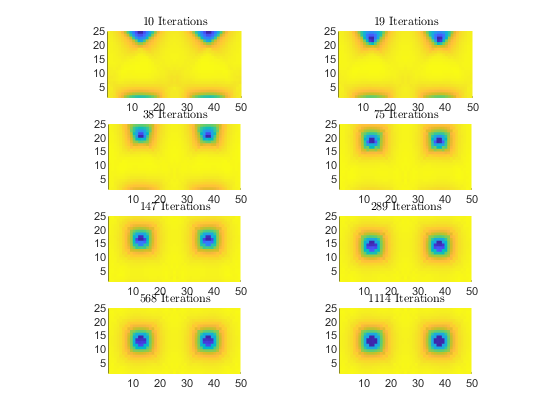
\includegraphics[width=\maxwidth{56.196688409433015em}]{figure_2.png}
\end{center}
\begin{center}
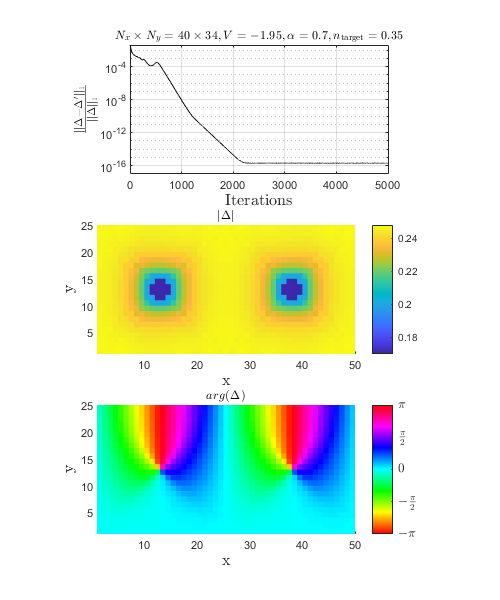
\includegraphics[width=\maxwidth{50.17561465127948em}]{figure_3.png}
\end{center}

\end{document}
